\section{Post-Training}


\subsection{Supervised Fine-Tuning}

We employ the Muon optimizer~\citep{jordan2024muon} in our post-training and recommend its use for fine-tuning with K2. This follows from the conclusion of our previous work~\cite{liu2025muon} that a Muon-pre-trained checkpoint produces the best performance with Muon fine-tuning.

We construct a large-scale instruction-tuning dataset spanning diverse domains, guided by two core principles: maximizing prompt diversity and ensuring high response quality. To this end, we develop a suite of data generation pipelines tailored to different task domains, each utilizing a combination of human annotation, prompt engineering, and verification processes.
We adopt K1.5~\citep{team2025kimi} and other in-house domain-specialized expert models to generate candidate responses for various tasks, followed by LLMs or human-based judges to perform automated quality evaluation and filtering.
For agentic data, we create a data synthesis pipeline to teach models tool-use capabilities through multi-step, interactive reasoning. 


\subsubsection{Large-Scale Agentic Data Synthesis for Tool Use Learning}
\label{sec:agentic-data-synthesis}

A critical capability of modern LLM agents is their ability to autonomously use unfamiliar tools, interact with external environments, and iteratively refine their actions through reasoning, execution, and error correction. Agentic tool use capability is essential for solving complex, multi-step tasks that require dynamic interaction with real-world systems. Recent benchmarks such as ACEBench~\citep{chen2025acebench} and $\tau$-bench~\citep{yao2024tau} have highlighted the importance of comprehensive tool-use evaluation, while frameworks like ToolLLM~\citep{qin2023toolllm} and ACEBench~\citep{chen2025acebench} have demonstrated the potential of teaching models to use thousands of tools effectively.

However, training such capabilities at scale presents a significant challenge: while real-world environments provide rich and authentic interaction signals, they are often difficult to construct at scale due to cost, complexity, privacy and accessibility constraints. Recent work on synthetic data generation (AgentInstruct~\citep{mitra2024agentinstruct}; Self-Instruct~\citep{wang2022self}; StableToolBench~\citep{guo2025stabletoolbenchstablelargescalebenchmarking}; ZeroSearch~\citep{sun2025zerosearchincentivizesearchcapability}) has shown promising results in creating large-scale data without relying on real-world interactions. Building on these advances and inspired by ACEBench~\citep{chen2025acebench}'s comprehensive data synthesis framework, we developed a pipeline that simulates real-world tool-use scenarios at scale, enabling the generation of tens of thousands of diverse and high-quality training examples.

\begin{figure}[t]
    \centering
    \begin{subfigure}[b]{0.4\textwidth}
        \centering
        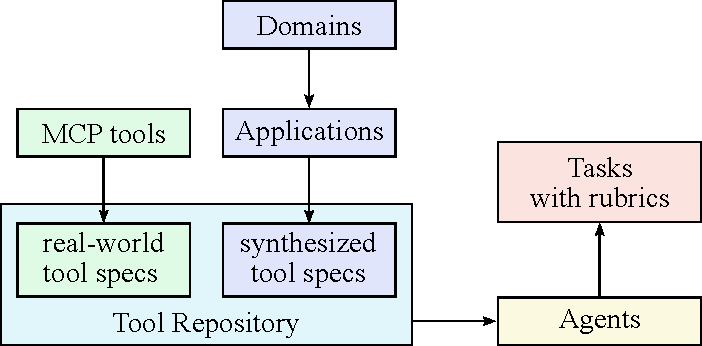
\includegraphics[width=\textwidth]{figures/tool_repo_synthesis.pdf}
        \caption{Synthesizing tool specs, agents and tasks}
        \label{fig:tool_repo_synth}
    \end{subfigure}
    \qquad
    \begin{subfigure}[b]{0.4\textwidth}
        \centering
        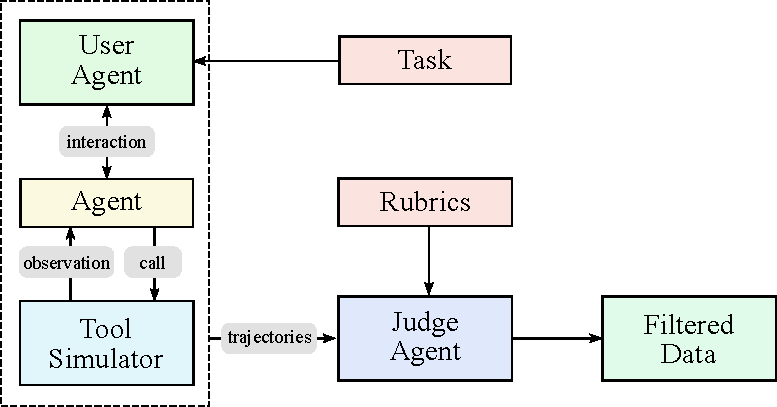
\includegraphics[width=\textwidth]{figures/tool_traj_synthesis.pdf}
        \caption{Generating agent trajectories}
        \label{fig:tool_traj_synth}
    \end{subfigure}
    \caption{Data synthesis pipeline for tool use. (a) Tool specs are from both real-world tools and LLMs; agents and tasks are the generated from the tool repo. (b) Multi-agent pipeline to generate and filter trajectories with tool calling.}
    \label{fig:tool_synth}
\end{figure}

\begin{figure}[t]
    \centering
    \begin{subfigure}[b]{0.48\textwidth}
        \centering
        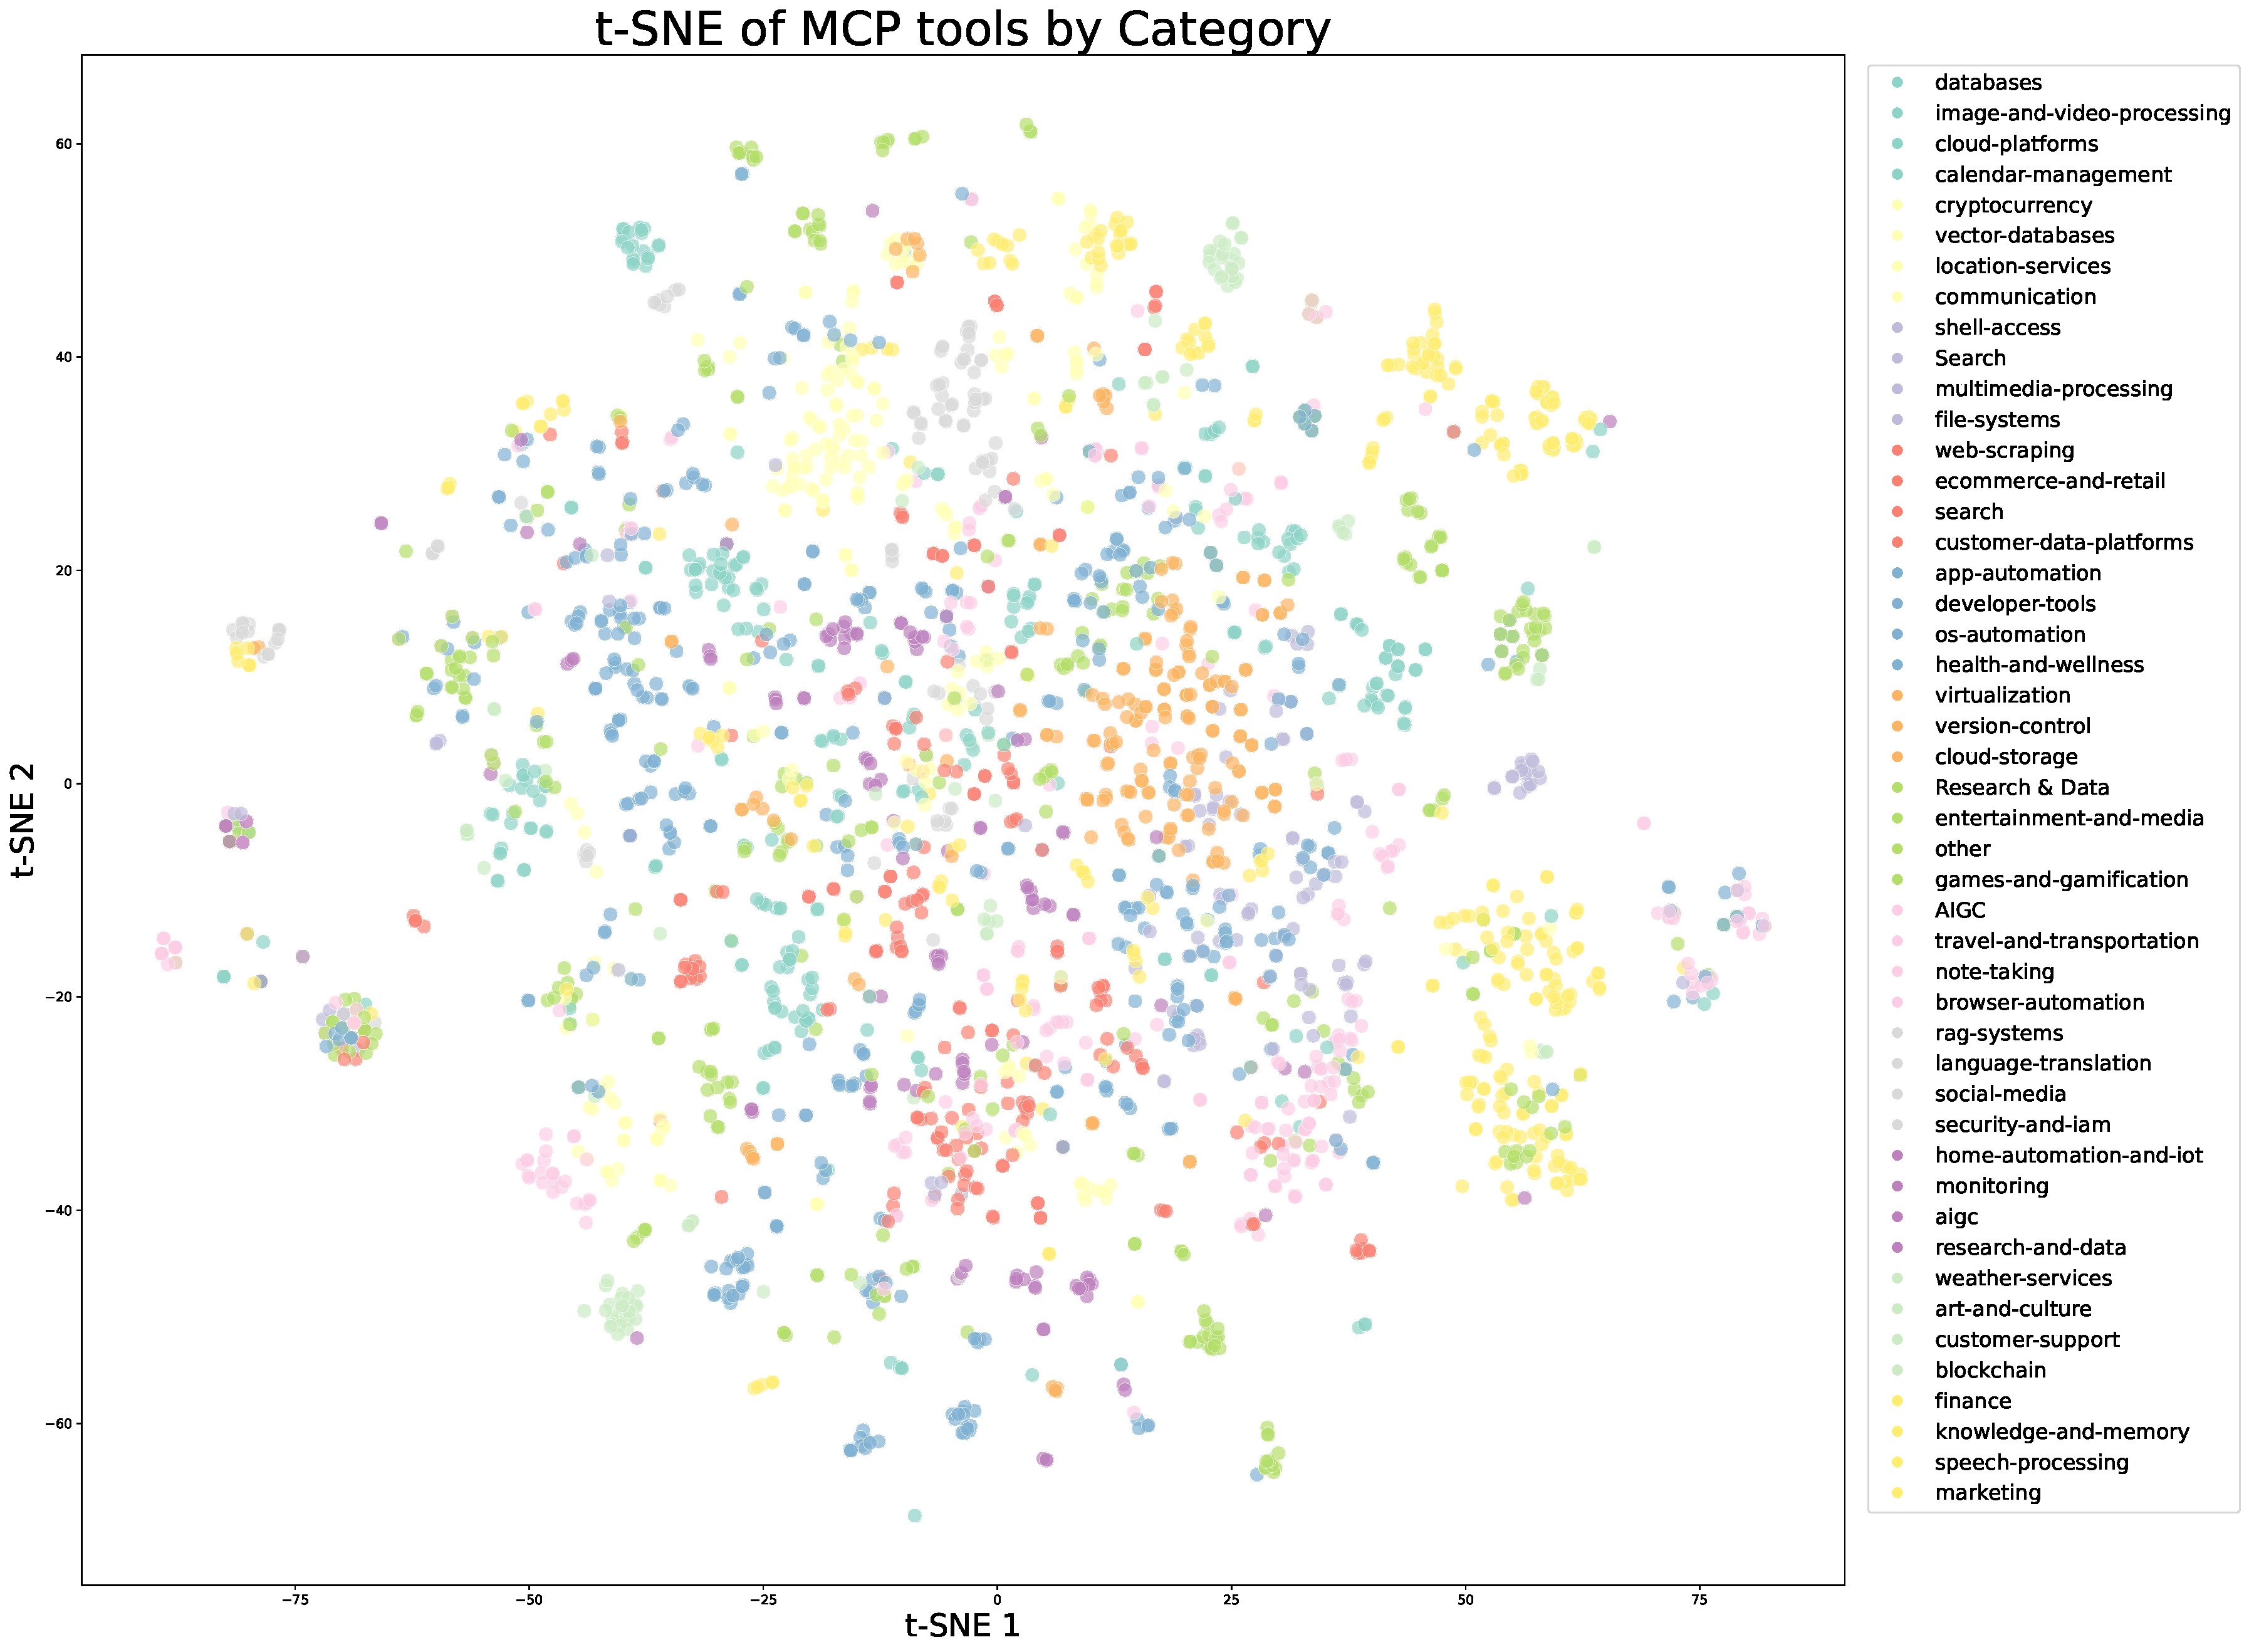
\includegraphics[width=\textwidth]{figures/tsne_tool_mcp.pdf}
        \caption{t-SNE visualization of real MCP tools, colored by their original source categories}
        \label{fig:tsne_mcp}
    \end{subfigure}
    \hfill
    \begin{subfigure}[b]{0.48\textwidth}
        \centering
        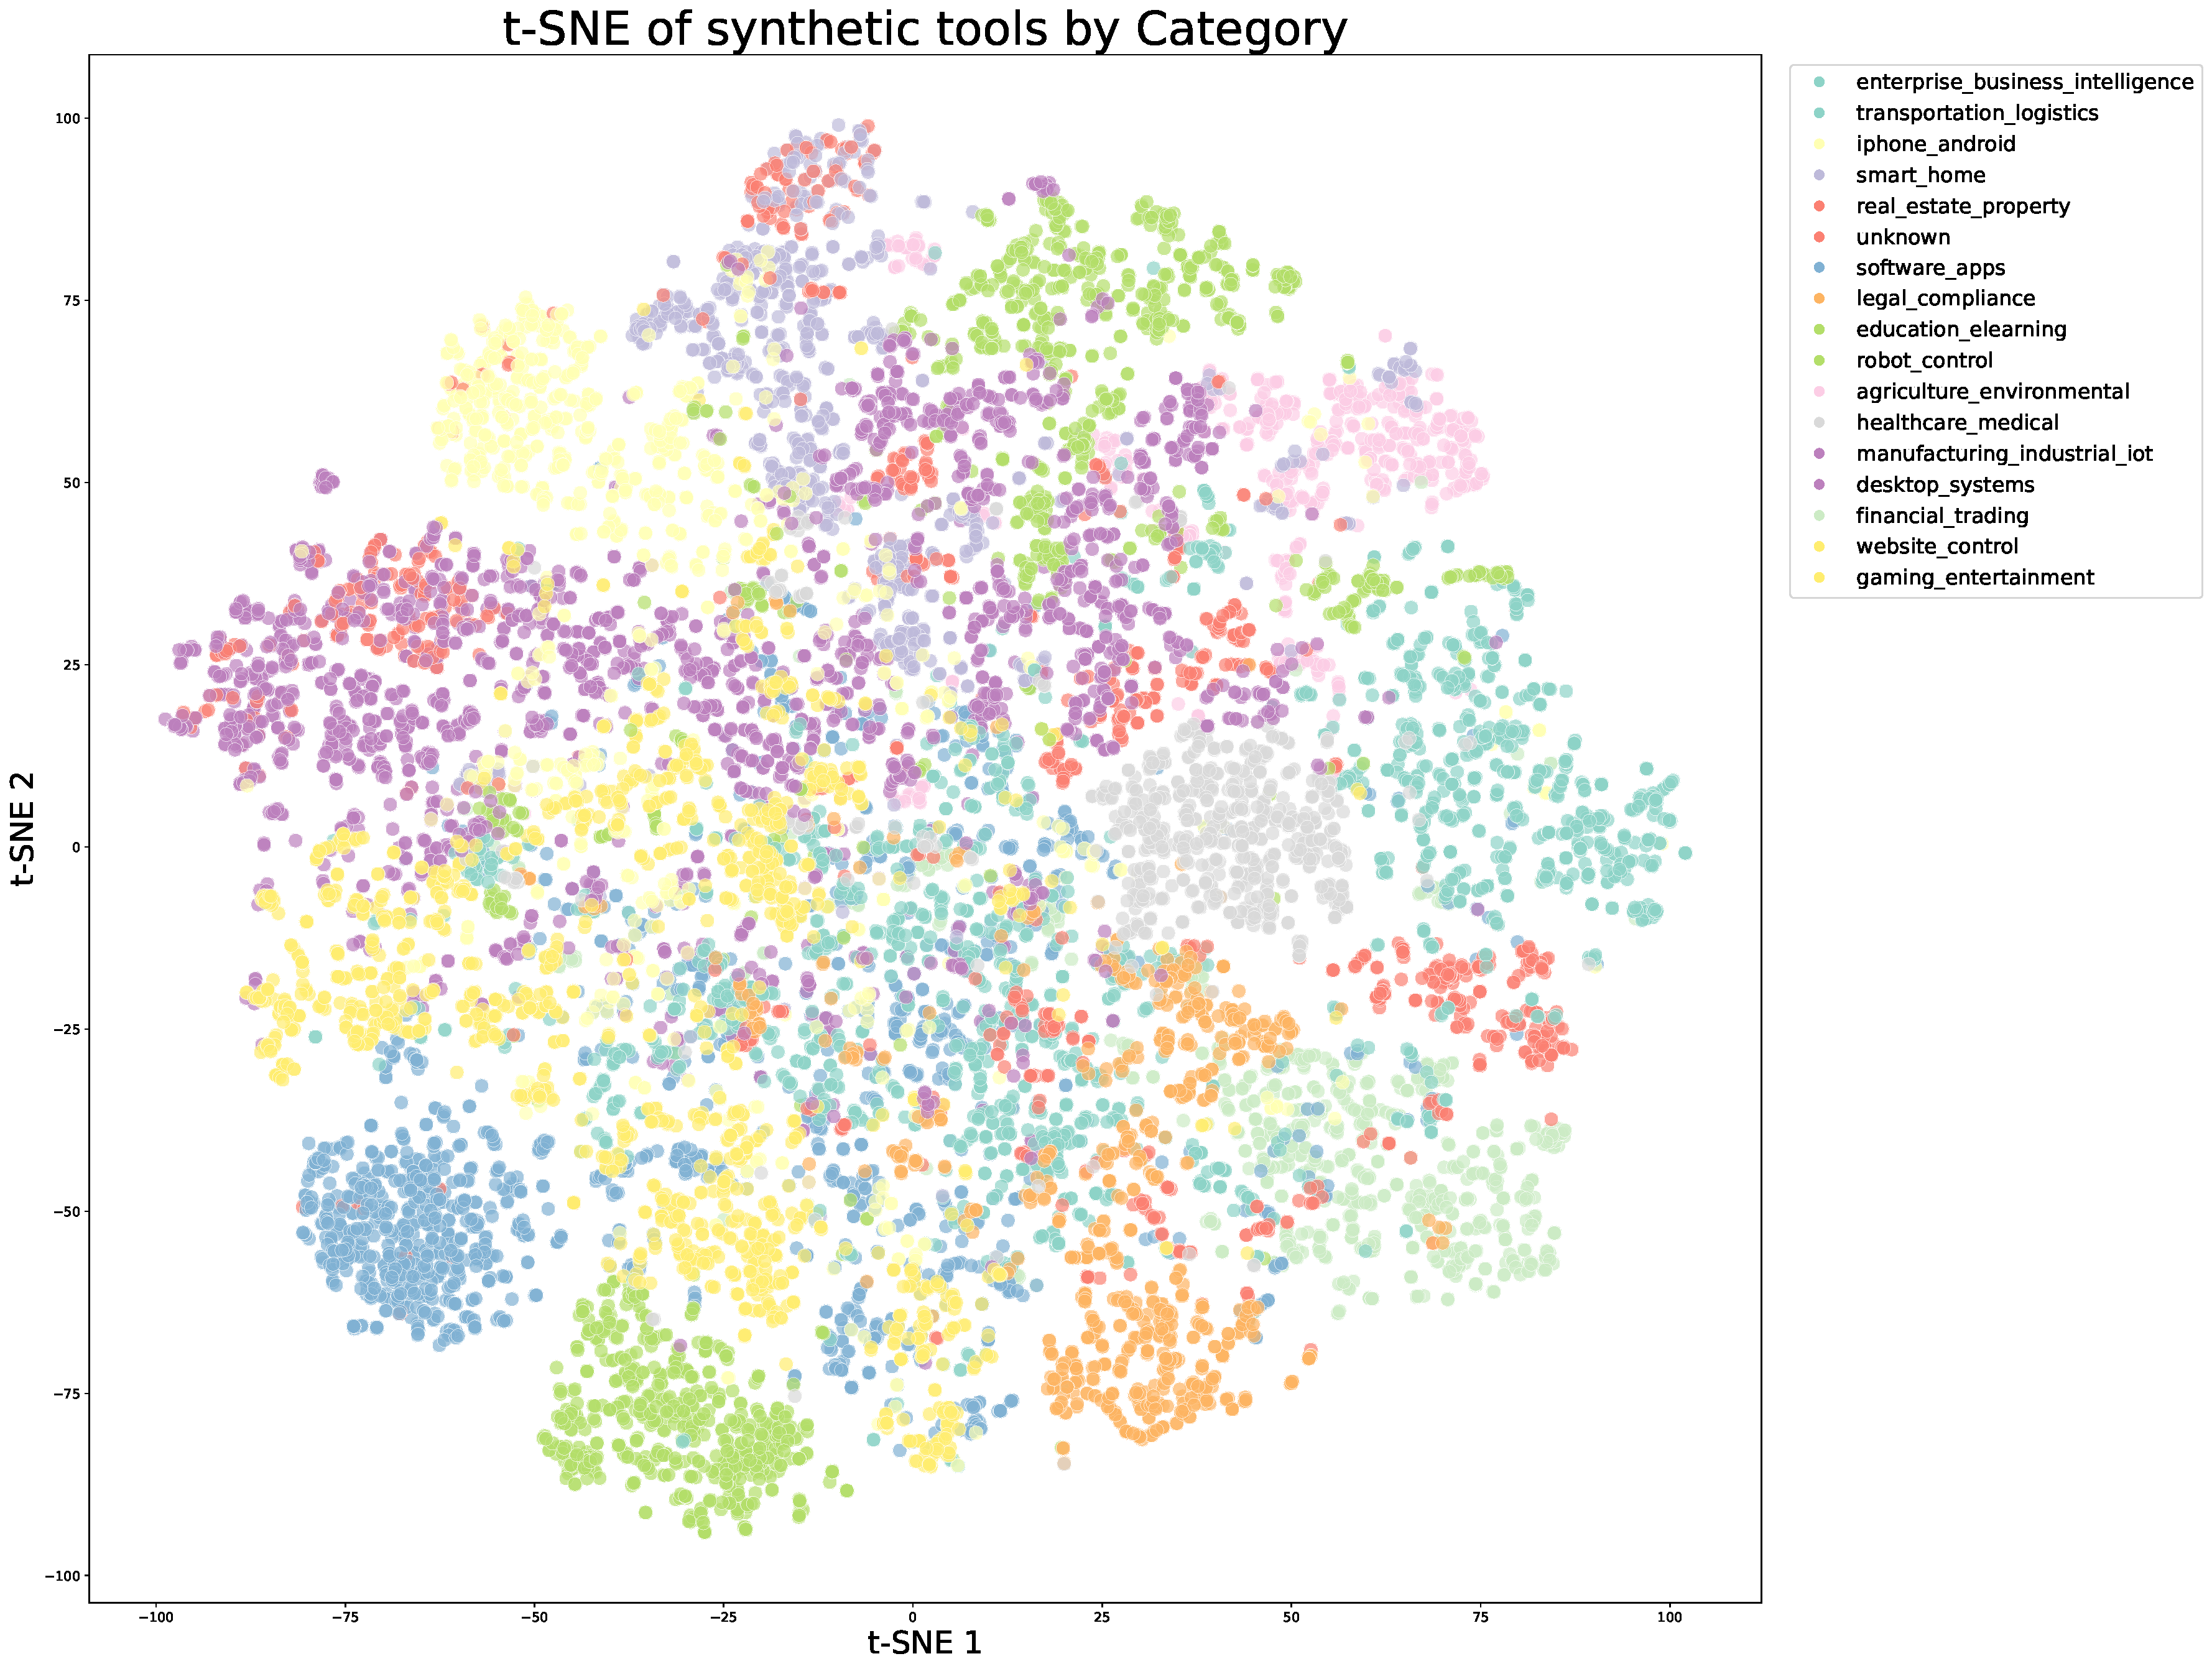
\includegraphics[width=\textwidth]{figures/tsne_tool_synthetic.pdf}
        \caption{t-SNE visualization of synthetic tools, colored by pre-defined domain categories}
        \label{fig:tsne_synthetic}
    \end{subfigure}
    \caption{t-SNE visualizations of tool embeddings. (a) Real-world MCP tools exhibit natural clustering based on their original source categories. (b) Synthetic tools are organized into pre-defined domain categories, providing systematic coverage of the tool space. Together, they ensure comprehensive representation across different tool functionalities.}
    \label{fig:tsne_tools}
\end{figure}

There are three stages in our data synthesis pipeline, depicted in Fig.~\ref{fig:tool_synth}.
\begin{itemize}
    \item \textit{Tool spec generation}: we first construct a large repository of tool specs from both real-world tools
    and LLM-synthetic tools;
    \item \textit{Agent and task generation}: for each tool-set sampled from the tool repository, we generate an agent to use the toolset and some corresponding tasks;
    \item \textit{Trajectory generation}: for each agent and task, we generate trajectories where the agent finishes the task by invoking tools.
\end{itemize}


\paragraph{Domain Evolution and Tool Generation.} We construct a comprehensive tool repository through two complementary approaches. First, we directly fetch 3000+ real MCP (Model Context Protocol) tools from GitHub repositories, leveraging existing high-quality tool specs. Second, we systematically evolve~\citep{xu2025wizardlmempoweringlargepretrained} synthetic tools through a hierarchical domain generation process: we begin with key categories (e.g., financial trading, software applications, robot control), then evolve multiple specific application domains within each category. Specialized tools are then synthesized for each domain, with clear interfaces, descriptions, and operational semantics. This evolution process produces over 20,000 synthetic tools. Figure~\ref{fig:tsne_tools} visualizes the diversity of our tool collection through t-SNE embeddings, demonstrating that both MCP and synthetic tools cover complementary regions of the tool space.

\paragraph{Agent Diversification.} We generate thousands of distinct agents by synthesizing various system prompts and equipping them with different combinations of tools from our repository. This creates a diverse population of agents with varied capabilities, areas of expertise, and behavioral patterns, ensuring a broad coverage of potential use cases.

\paragraph{Rubric-Based Task Generation.} For each agent configuration, we generate tasks that range from simple to complex operations. Each task is paired with an explicit rubric that specifies success criteria, expected tool-use patterns, and evaluation checkpoints. This rubric-based approach ensures a consistent and objective evaluation of agent performance.

\paragraph{Multi-turn Trajectory Generation.} We simulate realistic tool-use scenarios through several components:
\begin{itemize}
    \item \textit{User Simulation}: LLM-generated user personas with distinct communication styles and preferences engage in multi-turn dialogues with agents, creating naturalistic interaction patterns.
    \item \textit{Tool Execution Environment}: A sophisticated tool simulator (functionally equivalent to a world model) executes tool calls and provides realistic feedback. The simulator maintains and updates state after each tool execution, enabling complex multi-step interactions with persistent effects. It introduces controlled stochasticity to produce varied outcomes including successes, partial failures, and edge cases.
\end{itemize}

\paragraph{Quality Evaluation and Filtering.} An LLM-based judge evaluates each trajectory against the task rubrics. Only trajectories that meet the success criteria are retained for training, ensuring high-quality data while allowing natural variation in task-completion strategies.

\paragraph{Hybrid Approach with Real Execution Environments.} While simulation provides scalability, we acknowledge the inherent limitation of simulation fidelity. To address this, we complement our simulated environments with real execution sandboxes for scenarios where authenticity is crucial, particularly in coding and software engineering tasks. These real sandboxes execute actual code, interact with genuine development environments, and provide ground-truth feedback through objective metrics such as test suite pass rates. This combination ensures that our models learn from both the diversity of simulated scenarios and the authenticity of real executions, significantly strengthening practical agent capabilities.

By leveraging this hybrid pipeline that combines scalable simulation with targeted real-world execution, we generate diverse, high-quality tool-use demonstrations that balance coverage and authenticity. The scale and automation of our synthetic data generation, coupled with the grounding provided by real execution environments, effectively implements large-scale rejection sampling~\cite{huang2022large,zelikman2022star} through our quality filtering process. This high-quality synthetic data, when used for supervised fine-tuning, has demonstrated significant improvements in the model's tool-use capabilities across a wide range of real-world applications.



\subsection{Reinforcement Learning}
Reinforcement learning (RL) is believed to have better token efficiency and generalization than SFT.
Based on the work of K1.5~\citep{team2025kimi}, we continue to scale RL in both task diversity and training FLOPs in K2. To support this, we develop a Gym-like extensible framework that facilitates RL across a wide range of scenarios. We extend the framework with a large number of tasks with verifiable rewards. For tasks that rely on subjective preferences, such as creative writing and open-ended question answering, we introduce a self-critic reward in which the model performs pairwise comparisons to judge its own outputs. This approach allows tasks from various domains to all benefit from the RL paradigm. 

\subsubsection{Verifiable Rewards Gym}

\paragraph{Math, STEM and Logical Tasks}
For math, stem and logical reasoning domains, our RL data preparation follows two key principles, \emph{diverse coverage} and \emph{moderate difficulty}.

\emph{Diverse Coverage.} 
For math and stem tasks, we collect high-quality QA pairs using a combination of expert annotations, internal QA extraction pipelines, and open datasets~\citep{li2024numinamath,moshkov2025aimo}. During the collection process, we leverage a tagging system to deliberately increase coverage of under-covered domains. For logical tasks, our dataset comprises a variety of formats, including structured data tasks (e.g., multi-hop tabular reasoning, cross-table aggregation) and logic puzzles (e.g., the 24-game, Sudoku, riddles, cryptarithms, and Morse-code decoding).

\emph{Moderate Difficulty.} The RL prompt-set should be neither too easy nor too hard, both of which may produce little signal and reduce learning efficiency. We assess the difficulty of each problem using the SFT model's pass@k accuracy and select only problems with moderate difficulty.



\paragraph{Complex Instruction Following}
Effective instruction following requires not only understanding explicit constraints but also navigating implicit requirements, handling edge cases, and maintaining consistency over extended dialogues. We address these challenges through a hybrid verification framework that combines automated verification with adversarial detection, coupled with a scalable curriculum generation pipeline.
Our approach employs a dual-path system to ensure both precision and robustness:

\noindent\textit{Hybrid Rule Verification.} We implement two verification mechanisms: (1) deterministic evaluation via code interpreters for instructions with verifiable outputs (e.g., length, style constraints), and (2) LLM-as-judge evaluation for instructions requiring nuanced understanding of constraints. To address potential adversarial behaviors where models might claim instruction fulfillment without actual compliance, we incorporate an additional hack-check layer that specifically detects such deceptive claims.

\noindent\textit{Multi-Source Instruction Generation.} To construct our training data, we employ three distinct generation strategies to ensure comprehensive coverage: (1) expert-crafted complex conditional prompts and rubrics developed by our data team (2) agentic instruction augmentation inspired by AutoIF~\citep{dong2024selfplayexecution}, and (3) a fine-tuned model specialized for generating additional instructions that probe specific failure modes or edge cases. This multipronged approach ensures both breadth and depth in instruction coverage.

\paragraph{Faithfulness}

Faithfulness is essential for an agentic model operating in scenarios such as multi-turn tool use, self-generated reasoning chains, and open-environment interactions.
Inspired by the evaluation framework from FACTS Grounding~\citep{jacovi2025factsgroundingleaderboardbenchmarking}, we train a sentence-level faithfulness judge model to perform automated verification. The judge is effective in detecting sentences that make a factual claim without supporting evidence in context. It serves as a reward model to enhance overall faithfulness performance. 

\paragraph{Coding \& Software Engineering}

To enhance our capability in tackling competition-level programming problems, we gather problems and their judges from both open-source datasets~\citep{huang2025opencoderopencookbooktoptier,xu2025kodcodediversechallengingverifiable} and synthetic sources. To ensure the diversity of the synthetic data and the correctness of reward signals, we incorporate high-quality human-written unit tests retrieved from pre-training data. 

For software engineering tasks, we collect a vast amount of pull requests and issues from GitHub to build software development environment that consists of user prompts/issues and executable unit tests.
This environment was built on a robust sandbox infrastructure, powered by Kubernetes for scalability and security. It supports over 10,000 concurrent sandbox instances with stable performance, making it ideal for both competitive coding and software engineering tasks. 




\paragraph{Safety}
Our work to enhance the safety begins with a human-curated set of seed prompts, manually crafted to encompass prevalent risk categories such as violence, fraud, and discrimination.

To simulate sophisticated jailbreak attempts~(e.g., role-playing, literary narratives, and academic discourse), we employ an automated prompt evolution pipeline with three key components:
\begin{itemize}
    \item \textbf{Attack Model}: Iteratively generates adversarial prompts designed to elicit unsafe responses from the target LLM.
    \item \textbf{Target Model}: Produces responses to these prompts, simulating potential vulnerabilities.
    \item \textbf{Judge Model}: Evaluates the interaction to determine if the adversarial prompt successfully bypasses safety mechanisms.
\end{itemize}

Each interaction is assessed using a task-specific rubric, enabling the judge model to provide a binary success/failure label.



\subsubsection{Beyond Verification: Self-Critique Rubric Reward}

To extend model alignment beyond tasks with verifiable reward, we introduce a framework for general reinforcement learning from self-critic feedbacks. This approach is designed to align LLMs with nuanced human preferences, including helpfulness, creativity, depth of reasoning, factuality, and safety, by extending the capabilities learned from verifiable scenarios to a broader range of subjective tasks.  The framework operates using a \textit{Self-Critique Rubric Reward} mechanism, where the model evaluates its own outputs to generate preference signals. 
To bootstrap K2 as a competent judge, we curated a mixture of open-source and in-house preference datasets and initialize its critic capability in the SFT stage.

\paragraph{Self-Critiqued Policy Optimization}
In the first core process of the learning loop, the K2 actor generates responses for general prompts that cover a wide range of use cases. The K2 critic then ranks all results by performing pairwise evaluations against a combination of rubrics, which incorporates both \textit{core rubrics} (Appendix.~\ref{sec:k2-critic-creteria}), which represent the fundamental values of our AI assistant that Kimi cherish, prescriptive rubrics (Appendix.~\ref{sec:k2-must-not-creteria}) that aim to eliminate reward hacking, and \textit{human-annotated rubrics} crafted by our data team for specific instructional contexts. Although certain rubrics can be designated as mandatory, K2 retains the flexibility to weigh them against its internal priors. This capacity enables a dynamic and continuous alignment with its evolving on-policy behavior, ensuring that the model's responses remain coherent with its core identity while adapting to specific instructions.

\paragraph{Closed-Loop Critic Refinement and Alignment}
During RL training, the critic model is refined using verifiable signals. On-policy rollouts generated from verifiable-reward prompts are used to continuously update the critic, a crucial step that distills objective performance signals from RLVR directly into its evaluation model. This transfer learning process grounds its more subjective judgments in verifiable data, allowing the performance gains from verifiable tasks to enhance the critic's judgment on complex tasks that lack explicit reward signals. 
This closed-loop process ensures that the critic continuously recalibrates its evaluation standards in lockstep with the policy's evolution. By grounding subjective evaluation in verifiable data, the framework enables robust and scalable alignment with complex, non-verifiable human objectives. 

Consequently, this holistic alignment yields comprehensive performance improvements across a wide spectrum of domains, including user intent understanding, creative writing, complex reasoning, and nuanced language comprehension.

\subsubsection{RL Algorithm}

We adopt the policy optimization algorithm introduced in K1.5~\citep{team2025kimi} as the foundation for K2. 
For each problem $x$, we sample $K$ responses $\{y_1,\dots,y_k\}$ from the previous policy $\pi_{\mathrm{old}}$, 
and optimize the model $\pi_\theta$ with respect to the following objective: 
\begin{align*}
L_{\mathrm{RL}}(\theta) = \mathbb{E}_{x \sim\mathcal{D}}\left[ \frac{1}{K} \sum_{i=1}^K \left[  \left( r(x, y_i) - \bar{r}(x)- \tau \log \frac{\pi_\theta(y_i | x)}{{\pi}_{\mathrm{old}}(y_i | x)} \right)^2 \right]\right] \, ,
\label{eq:rl-objective}
\end{align*}
where $\bar{r}(x) = \frac{1}{k}\sum_{i=1}^k r(x, y_i)$ is the mean rewards of the sampled responses, $\tau>0$ is a regularization parameter that promotes stable learning. 
As in SFT, we employ the Muon optimizer~\citep{jordan2024muon} to minimize this objective. 
As we scale RL training to encompass a broader range of tasks in K2, a primary challenge is achieving consistent performance improvements across all domains. To address this, we introduce several additions to the RL algorithm. 


\paragraph{Budget Control}
It has been widely observed that RL often results in a substantial increase in the length of model-generated responses~\citep{team2025kimi,guo2025deepseek}. While longer responses can enable the model to utilize additional test-time compute for improved performance on complex reasoning tasks, the benefits often do not justify its inference cost in non-reasoning domains. 
To encourage the model to properly distribute inference budget, we enforce a per-sample \emph{maximum token budget} throughout RL training, where the budget is determined based on the type of task.  
 Responses that exceed this token budget are truncated and assigned a penalty, which incentivizes the model to generate solutions within the specified limit. Empirically, this approach significantly enhances the model's token efficiency, encouraging concise yet effective solutions across all domains.


\paragraph{PTX Loss} 

To prevent the potential forgetting of valuable, high-quality data during joint RL training, we curate a dataset comprising hand-selected, high-quality samples and integrate it into the RL objective through an auxiliary PTX loss~\citep{ouyang2022training}.
This strategy not only leverages the advantages of high-quality data, but also mitigates the risk of overfitting to the limited set of tasks explicitly present in the training regime. 
This augmentation substantially improves the model's generalization across a broader range of domains.

\paragraph{Temperature Decay}

For tasks such as creative writing and complex reasoning, we find that promoting exploration via a high sampling temperature during the initial stages of training is crucial. 
A high temperature allow the model to generate diverse and innovative responses, thereby facilitating the discovery of effective strategies and reducing the risk of premature convergence to suboptimal solutions. 
However, retaining a high temperature in the later stages of training or during evaluation can be detrimental, as it introduces excessive randomness and compromises the reliability and consistency of the model's outputs. 
To address this, we employ a temperature decay schedule, to shift from exploration to exploitation throughout the training. This strategy ensures that the model leverages exploration when it is most beneficial, while ultimately converge on stable and high-quality outputs.



























\subsection{RL Infrastructure}

\subsubsection{Colocated Architecture}
Similar to K1.5~\citep{team2025kimi}, we adopt a hybrid colocated architecture for our synchronized RL training, where the training and inference engines live on the same workers. When one engine is actively working, the other engine releases or offloads its GPU resources to accommodate. In each iteration of RL training, a centralized controller first calls the inference engine to generate new data for training. It then notifies the training engine to train on the new data, and send updated parameters to the inference engine for the next iteration. 

Each engine is heavily optimized for throughput. In addition, as the model scales to the size of K2, the latency of engine switching and failure recovery becomes significant. We present our system
design considerations in these aspects.

\subsubsection{Efficient Engine Switching}

During rollout, the parameters of the training engine are offloaded to DRAM. Bringing up the training engine is therefore a simple step of H2D transmission. 
However, bringing up the inference engine is a bigger challenge, as it must obtain updated parameters
from the training engine with a different
sharding paradigm.

\begin{figure}
    \centering
    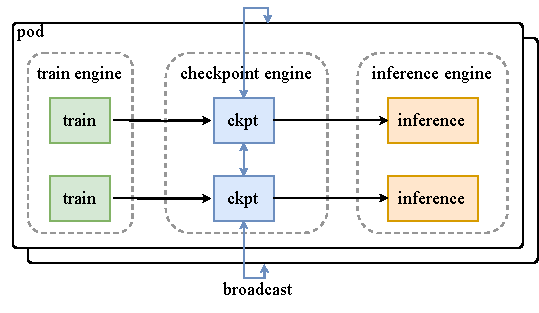
\includegraphics[width=0.5\linewidth]{figures/rl-ipc.drawio.pdf}
    \caption{Parameter update utilizing a checkpoint engine}
    \label{fig:RL-weight}
\end{figure}

Given the scale of K2 and the vast number of devices involved, using a network file system for resharding and broadcasting parameters is impractical. The aggregate bandwidth required to keep overhead low reaches several petabytes per second. To address this challenge, we developed a distributed checkpoint engine co-located on training nodes to manage parameter states. To perform a parameter update, each checkpoint engine worker obtains a local copy of parameters from the training engine, then broadcasts the full parameter set across all checkpoint engine workers. Subsequently, the inference engine retrieves only the parameter shard it requires from the checkpoint engine. This process is illustrated in Figure~\ref{fig:RL-weight}. To enable this for a 1T model, updates are performed parameter-by-parameter in a pipelined manner, minimizing memory footprint (see Appendix~\ref{sec:k2-rl-update-appendix}). 

We opt to broadcast the full parameter set across the entire cluster, regardless of the specific sharding schemes on each inference worker. While this transfers several times more data than a theoretically optimal approach, it offers a simpler system design that is less intrusive to the training and inference engines. We chose to trade off this minor overhead to fully decouple the training engine and the inference engine, significantly simplifying maintenance and testing. 

Notably, this approach outperforms the transfer-what-you-need method due to reduced synchronization overhead and higher network bandwidth utilization.
Our system can complete a full parameter update for Kimi K2 with less than 30 seconds, a negligible duration for a typical RL training iteration. The source code for the checkpoint engine is available on Github\footnote{\url{https://github.com/MoonshotAI/checkpoint-engine}}.




\subsubsection{Efficient System Startup}

As large-scale training is prone to system failure, optimizing the startup time is crucial for models as large as Kimi K2.

To start the training engine, we let each training worker selectively read part or none of the parameters from disk, and broadcast necessary parameters to its peers. The design goal is to ensure all workers collectively read the checkpoint only once, minimizing expensive disk IO. 

As the inference engines are independent replicas, we would like to avoid introducing extra synchronization barriers between them. Therefore, we opt to reuse checkpoint engine for startup: we let checkpoint engine collectively read the checkpoint from disk, similar to how the training engine starts. Then it updates the state of the uninitialized inference engine, using the approach introduced in the previous section. By leveraging the dedicated checkpoint engine, the system also becomes robust to single-point failures, because an inference replica can restart without communicating with other replicas.




\subsubsection{Agentic Rollout}
Our RL infrastructure supports the training of long-horizon, multi-turn agentic tasks. During rollout, these tasks present distinct challenges, such as complex environmental interactions and prolonged rollout durations. Here we introduce a few optimizations to alleviate these issues.

Due to the diversity of environments, certain interactions may be blocked on waiting for environment feedback (e.g., a virtual machine or a code interpreter), leaving the GPUs idle. We employ two strategies to maximize GPU utilization: (i) we deploy heavy environments as dedicated services that can scale up more easily; (ii) we employ a large number of concurrent rollouts to amortize the latency induced by certain expensive interactions.

Another challenge in agentic rollout is that individual rollout trajectories can be extremely long. To prevent long-tail trajectories from blocking the entire rollout process, we employ the partial rollout~\citep{team2025kimi} technique. This strategy allows long-tail unfinished tasks to be paused, and resumed in the next RL iteration.

To improve research efficiency, we also design a unified interface inspired by the OpenAI Gym framework~\citep{openaigym2016} to streamline the integration of new environments. We hope to scale our RL infrastructure to more diverse interactive environments in the future.